\documentclass[11pt]{report}
\usepackage[utf8]{inputenc}
\usepackage[danish]{babel}
\usepackage [T1]{fontenc}
\usepackage[margin=2.5cm]{geometry}
\usepackage[hidelinks]{hyperref}
\usepackage{graphicx}
\graphicspath{{Img/}}
\usepackage{listings}
\usepackage{color}
\usepackage{adjustbox}
\usepackage{tocloft}
\usepackage{listings}
\usepackage{enumitem}
\usepackage{indentfirst}
\usepackage{caption}
\usepackage{float}

\setlength{\parskip}{12pt}

\definecolor{dkgreen}{rgb}{0,0.6,0}
\definecolor{gray}{rgb}{0.5,0.5,0.5}
\definecolor{mauve}{rgb}{0.58,0,0.82}

\lstset{frame=tb,
  language=Java,
  aboveskip=3mm,
  belowskip=3mm,
  showstringspaces=false,
  columns=flexible,
  basicstyle={\small\ttfamily},
  numbers=none,
  numberstyle=\tiny\color{gray},
  keywordstyle=\color{blue},
  commentstyle=\color{dkgreen},
  stringstyle=\color{mauve},
  breaklines=true,
  breakatwhitespace=true,
  tabsize=3
}

\definecolor{bluekeywords}{rgb}{0.13,0.13,1}
\definecolor{greencomments}{rgb}{0,0.5,0}
\definecolor{turqusnumbers}{rgb}{0.17,0.57,0.69}
\definecolor{redstrings}{rgb}{0.5,0,0}


\lstdefinelanguage{FSharp}
                {morekeywords={let, new, match, with, rec, open, module, namespace, type, of, member, and, for, in, do, begin, end, fun, function, try, mutable, if, then, else},
    keywordstyle=\color{bluekeywords},
    sensitive=false,
    morecomment=[l][\color{greencomments}]{///},
    morecomment=[l][\color{greencomments}]{//},
    morecomment=[s][\color{greencomments}]{{(*}{*)}},
    morestring=[b]",
    stringstyle=\color{redstrings}
    }
\usepackage{amsmath}

\title{Social Engineering\\Security}
\author{
Asger H. Sørensen\\
\\cph-as466
\and
William S. Huusfeldt\\
\\cph-wh106
\and
Emil J. Svensmark\\
\\cph-eb122
}
\date{29 - maj - 2020}
\begin{document}
\maketitle
\renewcommand{\cftchapleader}{\cftdotfill{\cftdotsep}}
\tableofcontents
\newpage

\chapter*{1. Indledning}
\addcontentsline{toc}{chapter}{1. Indledning}
Denne rapport vil omhandle et ofte overset område af cybersikkerhed: den humane faktor. I denne rapport indgår eksempler på phishing og vishing ved at analysere firmaers og privates håndtering af det, når det forekommer. Der vil blive lavet test-baseret vishing forsøg på virksomheder og test-baseret phishing forsøg på private folk, hvorefter handlingerne på dem, hver i sær vil blive analyseret. I rapporten vil disse handlinger og forbehold også blive diskuteret samt eventuelt komme med løsninger/ændringer med målet om at øge sikkerheden, hvis den ikke skulle være tilstrækkelig. Hvis den skulle vise sig at være tilstrækkelig, så vil der diskuteres hvilke forhold der gør at sikkerheden er stærk nok. 

\chapter*{2. Sikkerhed}
\addcontentsline{toc}{chapter}{2. Sikkerhed}

\section*{2. 1 Den Humane Faktor}
\addcontentsline{toc}{section}{2. 1 Den Humane Faktor}
I starten af det 21. århundrede så man en udvikling verden over med øget kulturel og økonomiske veksling på kryds og tværs af landegrænser. Det er i de første årtier af dette århundrede, hvor globaliseringen for alvor kan mærkes. Virksomheders grænser og rækkevidde er blevet mindre synlige og sværere at håndtere, hvorfor også infrastrukturen åbnes op for nye svagheder og udfordringer. Som teknologien udvikler sig, vil sikkerhedstrusler modnes og blive en del af hverdagen.

Den tidligere direktør for FBI, Robert Mueller sagde “There are only two types of companies: those that have been hacked, and those that will be.” Denne udtalelse rummer en ildevarslende pessimisme, som viser hvor betydeligt et omfang cybersikkerhed har udviklet sig til. Det er ikke ualmindeligt at se personer, uden ekspertise i computere, som besidder kritiske positioner i en infrastruktur; f.eks. bankrådgivere med persondata på kunder og sygeplejersker i sundhedssektoren.


I applikationer, som forskellige erhverv benytter sig af i sin dagligdag, kan det være svært at beskytte sig mod insider attacks, et angreb der forekommer “bag muren” af firmaet af en (tidligere) ansat for eksempel, både økonomisk og teknisk. Men disse risici kan imødekommes med sikkerhedsstyring. Brugen af sikkerheds teknologi er i stigende grad nødvendig, såsom firewalls og autentificering, som beskytter mod uautoriseret adgang.


Et område er dog ofte glemt i ligningen om cybersikkerhed, hvilket er det menneskelige aspekt. Gennem social engineering teknikker kan ondsindede bryde organisatoriske sikkerhed gennem sociale interaktioner. 

\section*{2. 2 Social Engineering}
\addcontentsline{toc}{section}{2. 2 Social Engineering}
   2. 2 Social engineering
Udvikling af nye teknologier, forbedringer af eksisterende IT løsninger og mere robuste krypteringsværktøjer har betydet, at hackere må se til gammeldags metoder. Her kommer social engineering ind på banen. Det er banalt sagt en psykologisk manipulationsteknik, hvor formålet er at fremtvinge en respons fra et mål(firma, person), som ikke er i vedkommendes bedste interesse og dermed tvinge vedkommende i en udsat position.

Oftest ses brugen af social engineering med formålet at influere en entitet til at udføre en handling. Dette kan være så simpelt som en phishingmail(mere om dette senere), hvor en bruger vildledes med et link til en side, som potentielt kan logge brugerens oplysninger.


I stigende grad er dette et problem. Ifølge KnowBe4 er kun omkring 3 procent af malware forsøg baseret på at udnytte tekniske mangler/fejl, hvor de andre 97 procent er forsøg på at narre brugere ved brug af social engineering teknikker.\footnote{\url{https://www.knowbe4.com/what-is-social-engineering/}}


En FBI undersøgelse viste, at BEC (Business Email Compromise) kostede virksomheder i 131 lande omkring fem milliarder USD mellem 2013-2016.\footnote{\url{https://www.trendmicro.com/vinfo/pl/security/news/cybercrime-and-digital-threats/billion-dollar-scams-the-numbers-behind-business-email-compromise}} Dette tal har udviklet sig voldsomt, hvor FBI pr. juli 2019, estimerede tab på over 26 milliarder USD på verdensplan.\footnote{\url{https://www.ic3.gov/media/2019/190910.aspx}}  Disse tal er endvidere kun baseret på indberettede oplysninger - dermed kan tallene være højere.
\begin{figure}[H]
  \center{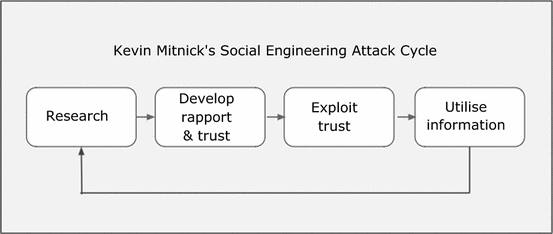
\includegraphics[height=6.2cm, width=15cm]
  {AttackCycle}}
  \caption*{Figur 1: Kevin Mitnicks SE angrebscyklus }
\end{figure}


I ovenstående model illustrerer Kevin Mitnick de fire faser der indgår i et Social Engineering angreb. Første fase foregår før angrebet er iværksat. Her undersøger angriberen sit offer, hvilke svagheder har denne? Hvilken information er vigtig i forhold til angrebet. Det er her hvor angriberen finder sin indgangsvinkel på ofret.
I anden fase vil angriberen forsøge at etablere tillid mellem ham og ofret til senere brug i angrebets tredje fase, hvor den selv samme tillid bliver udnyttet. 
Det er i tredje fase hvor angriberen forsøger at anskaffe information eller få offeret til at udføre en ønsket handling. 
I det fjerde og sidste stadie af angrebet vil al information og andre ressourcer som er anskaffet blive brugt for at opnå det ønskede resultat.

\section*{2. 3 Beskyttelse mod social engineering angreb}
\addcontentsline{toc}{section}{2. 3 Beskyttelse mod social engineering angreb}
Som følge af den stigende hyppighed af denne type angreb, er det i stigende grad nødvendigt at adressere hvordan man forsvarer sig. På baggrund af, at social engineering omhandler manipulation af mennesker, må antagelsen være, at vedkommende selv må forholde sig kritisk til f.eks. en mail fra en ukendt person der beder om at klikke på et link, eller en organisation der fortæller at man har vundet en gevinst der ligeledes linker til en side, kan være falsk og et forsøg på hacking.
FBI anbefaler i sin sektion om, hvordan man beskytter sig selv mod BEC scams, at man benytter sig af to-faktor autentificering på alle konti der tillader det.\footnote{\url{https://www.fbi.gov/scams-and-safety/common-scams-and-crimes/business-email-compromise}} Denne foranstaltning kan også være tvungen i organisationer. Ydermere nævner FBI også at man skal være opmærksom og kritisk over for hvilken information om sig selv man åbent deler på sociale medier; information som fødselsdato, familiemedlemmer, skoler, etc.

Et studie viser at 59\% af amerikanere har benyttet sig af et kodeord med en fødselsdato\footnote{\url{https://dataprot.net/statistics/password-statistics/}}, hvorfor den information kan være essentiel for en hacker - endnu mere taget i betragtning, at et kodeord i gennemsnit bliver brugt på fem forskellige konti.

En organisation kan have nok så mange firewalls og et intrusion detection system oppe at køre, men hvilken nytte har dette, hvis en medarbejder videregiver sine loginoplysninger i et social engineering angreb? Svaret er: Knap så meget nytte.


Ifølge FBI, så er alt i alt det som en organisation kan gøre udover beskyttelse med firewalls etc. at træne og uddanne sine medarbejdere til at tage ekstra forbehold og være varsomme med deres egne data.

\section*{2. 4 Phishing og man-in-the-middle}
\addcontentsline{toc}{section}{2. 4 Phishing og man-in-the-middle}
Phishing er metode til at udnytte huller i et sikkerhedssystem der ikke håndterer sikkerheden godt nok i forhold til når en person udgiver sig for at være ejeren af en andens konto/firma. Et oplagt eksempel på phishing ville være at nogen udgiver sig for at være en nigeriansk prins som vil sende nogle penge mod et startbeløb, men blot ender med at løbe afsted med de penge der blev modtaget. 


Dette er dog ret forældet, og et mere nutidigt eksempel på et phishing angreb, som mange ældre personer ofte falder for, ville være når en person udgiver sig for at være et anerkendt firma, som “udgiver gratis præmier”. Så snart at ofret har klikket på linket for at få deres præmie, er skaden dog typisk allerede sket, da der nu er en mulig man-in-the-middle forbindelse eller andre former for angreb. En man-in-the-middle er teoretisk set en person der kan sidde hemmeligt og overvåge en anden persons forbindelse med en server.


Den bedste måde for at afværge disse angreb, er at ignorere alle former for links og beskeder man ikke kender til. På trods af denne åbenlyse løsning, er der stadig mange der falder i.
\section*{2. 5 Vishing}
\addcontentsline{toc}{section}{2. 5 Vishing}
Vishing her er en metode der udnytter huller i et sikkerhedssystem som ikke håndterer sikkerheden ordentligt, når det kommer til folk der udgiver sig for at være andre. Den store forskel på phishing og vishing er dog at modsat phishing, som forekommer over beskeder, mails og andet tekstbaseret kommunikation, så forekommer visning over mundtligt kommunikation. Dette gør det muligt at udnytte offeret langt nemmere, da det er meget nemmere at overbevise offeret om at man er en anden person over mundtlig kommunikation.

Vishing kan udføres på to forskellige måder, og med to forskellige interessenter i tanke. 

\noindent\textbf{Personlig/Identitets Vishing}
\par Angriberen har undersøgt sit offer meget, og har prøvet at finde så meget som muligt offentligt information på offeret. Angriberen kan også have prøvet at få fat i ikke offentlige informationer ved brug af et andet angreb. Når nok information er indsamlet om offeret, kontakter angriberen offerets virksomhed til den konto angriberen vil have adgang til. 

Dette gøres for det meste for at udføre skade til et enkelt individ, af enten politiske årsager, had/hævn, eller andre personlige årsager.

Et eksempel på dette ville være at en person udgiver sig for at være en stresset forældre med et grædende barn i armene som bare har mistet sit password og skal have et reset. I virkeligheden er det en person der blot sætter en lydfil af en baby til at køre i baggrunden og imens lyder overbevisende nok til at virke stresset.

\noindent\textbf{Ikke-personlig Vishing}
\par Her bliver en person ringet op af en der udgiver sig for at være repræsentant af et firma. Det mest kendte eksempel af dette er en indisk mand der ringer for at fortæller at der er noget galt med ens computer/mac. Her udgiver personen sig for at ville hjælpe dig, og at de har opfanget virus eller anden årsag til kontakt og vil hjælpe dig med at fjerne det. Det som angriberen gerne vil opnå dog er noget helt andet, og hvad angriberen vil opnå kan variere meget. Angriberen kan have interesse i flere ting på din private computer; som private oplysninger (bank numre, passwords, e-mails osv.), men også mulighed for fjernstyring eller overvågning. 
\chapter*{3. Forsøg}
\addcontentsline{toc}{chapter}{3. Forsøg}

\section*{3. 1 Beskrivelse \& Formål}
\addcontentsline{toc}{section}{3. 1 Beskrivelse \& Formål}
\noindent\textbf{Vishing}
\par Formålet med forsøget om vishing er at teste hvorvidt man kan få adgang til en andens konto ved at ringe til et firma, få adgang til kontoen og ændre koder og e-mail til kontoen uden at være ejer af den. Ud fra resultaterne vil vi gennemgå hvad for nogle sikkerhedsforanstaltninger firmaer har for at undgå dette, og hvis der var nogen mangler på sikkerhedsforanstaltninger.


\noindent\textbf{Phishing}
\par Formålet med forsøget om visning er at teste om hvorvidt man kan få folk til at klikke på links de ikke bør klikke på. Ud fra resultaterne vil der diskuteres om hvilke forbehold folk bør tage hver eneste gang de får tilsendt et link eller lignendende. Dette forsøg vil prøve at fordele aldersgruppen til to segmenter, hvoraf det ene segment er mennesker i alderen mellem 20-28, og det andet segment er mennesker i alderen mellem 50-80. Vi vil se hvorvidt man kan se hvem der er mere tilbøjelige til at trykke på phishing links. 

\section*{3. 2 Fremgangsmåde}
\addcontentsline{toc}{section}{3. 2 Fremgangsmåde}
\noindent\textbf{Vishing}
\par For at kunne prøve at få fat på en konto, uden at man selv er ejer af den er der en del forberedelse der skal gøres først. Offeret blev slået op på de gule sider og krak, hvoraf vi fik et telefonnummer samt adresse på offeret. Derefter blev offerets sociale medier, herunder Facebook og instagram gået igennem for at finde information om offeret der kunne have relevans for angrebet. Til sidst blev en ny mail oprettet, som skulle ligne en privat mail som offeret i forsøget kunne have haft.

Som en anden forberedelse, var der mege diskussion om hvorvidt dette var lovligt, på trods af at “offeret” var involveret og havde sagt god for forsøget. Derfor for at være på den sikre side skrev vi en kontrakt, som alle i gruppen underskrev. Dette var en måde at vise at der var givet tilladelse, på trods af den gråzone som forsøget skulle forekomme i.

\noindent\textbf{Phishing}
\par Phishing forsøget startede med at der blev oprettet en Maven side på en af vores servere. Det eneste der står på siden er, at vi er i gang med et eksamensprojekt, og advarer folk om at de skal være påpasselige med, hvad for nogle links folk trykker på. 
\begin{center}
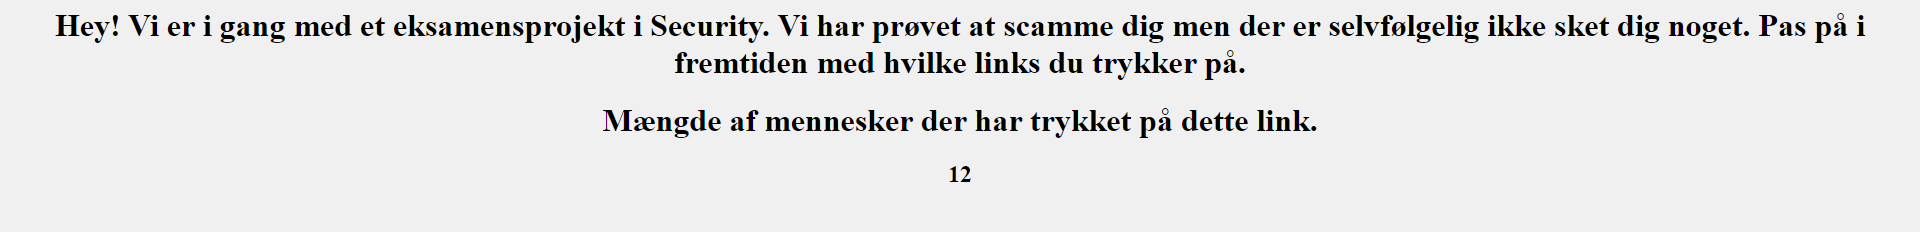
\includegraphics[height=3cm, width=17cm]{Capture}
\end{center}
I dette eksempel har vi udgivet os for at være Elgiganten, hvor vi har sendt en besked ud omkring at pågældende person har vundet en konkurrence om et gavekort til 2500 kr. Der skal blot trykkes på linket til at få indløst gavekortet, som så fører til vores side som tæller indexet op en gang. Mailen bliver sendt fra en nyoprettet email konto noreply.elgiganten.teknik@gmail.com, som blev brugt til at sende mails til mennesker som vi selv kender, således at mailen ikke kommer ud til fremmede mennesker. 
\begin{center}
\includegraphics[height=18cm, width=17cm]{Phishing-Email}
\end{center}
Vi har været påpasselige med hvem vi har sendt mails til, da der er nogle der bor sammen med andre. Vi har kun sendt en mail per husstand, for at virke mindre suspekt. Billederne er taget direkte fra elgigantens hjemmeside for at få det til at ligne så tæt på en original mail som muligt, med inkluderet betingelser i småt i bunden af mailen, samt reklame tilbud. 

Vi har prøvet at kontakte rigspolitiets NC3 afdeling for at forhøre os om lovgivning angående dette forsøg, da vi ikke selv har kunnet finde noget specifikt der siger dette i mod. Vi har ikke hørt fra NC3 angående tilladelse, og har derfor begrænset forsøget en del for at teste inden for lovens rammer. 

\section*{3. 3 Resultat}
\addcontentsline{toc}{section}{3. 3 Resultat}
\noindent\textbf{Vishing}
\par Angreb forekom som følgende: Emil’s telefonselskabs nummer bliver slået op og ringet til, hvorefter man bliver modtaget af en automatisk respons, der beder om at specificere om hvad opkaldet drejer sig om. Computeren beder først om telefonnummeret opkaldet drejer sig om. Derefter beder computeren en om at indtaste cpr nummeret der er tilknyttet til kontoen. 
	
Her kom første problem, da cpr nummer ikke normalt er noget man har adgang til hos en person man ikke kender. Vi lod være med at oplyse noget som helst, i håb om at der ville ske noget alligevel - hvilket der gjorde. Man bliver viderestillet til personalet, hvis man ikke angiver et cpr nr. hvilket er det som vi ønsker; mundtligt kommunikation.
Vi kommer i kontakt med personalet, som vi fortæller, at vi ikke kan få adgang til kontoen, hvis man ikke kan oplyse det cpr. nummer der er tilknyttet den nævnte konto. Det er her social engineering kommer ind i billedet, for hvis vi kan overbevise personalet om at vi af en eller anden grund ikke har mulighed for at oplyse cpr. nummeret, kan vi muligvis få adgang til kontoen alligevel.
	
Som svar på spørgsmålet om cpr. nummeret, så siger vi, at vi har glemt det, og at vores pung og mobil lige er blevet stjålet, både grunden til at vi ønsker at ændre nogle oplysninger, men også en årsag til at vi ikke har adgang til cpr nummeret. På trods af at vi insisterer, insisterer personen selv på at det ikke er muligt, og at deres system ikke tillader det.

\noindent\textbf{Phishing}
\par Efter at have sendt mailen ud og ventet længe nok på, at vi kan vurdere at folk har set den, og enten har klikket eller valgt at ignorere mailen, endte resultatet med at der var ca. 25 klik på linket. Vi har ikke taget højde for om folk har klikket flere gange på linket, som er en reel mulighed, og derfor kan tallet være en smule misvisende.


Vi har efter dette forsøg haft kontakt med nogle af de udsatte. En af dem vi har snakket med var en mor af en fra gruppen, som endte med at klikke på linket. Vi spurgte ind til om hvad der fik hende til at klikke, og svaret gik på at “jeg gik ikke ud fra der var en fare ved det, da jeg ikke forinden havde opgivet nogle oplysninger”-


Derudover var der flere personer der endte med ignorere det, samt en der var ved at rapportere mailen. Da vi spurgte en af personerne der valgte at ignorere mailen om hvorfor de valgte ikke at trykke på linket, fik vi afvide at “det skyldes at jeg så at det var en gmail, og var derfor nok ikke tilknyttet det firma (Elgiganten) som det udgav sig for at være”. En anden person der valgte at ignorere linket, og var ved at rapportere mailen, var en yngre person, modsat de to andre. Hans svar til hvorfor; var at “jeg altid tjekker linket, og da jeg så sidens domæne, vidste jeg med det samme at det var usikkert” - han kom også frem til at det nok var os der havde sendt det, på trods af vi udelukkende havde bedt om hans mail dagen i forvejen uden andet info. Derudover var der flere der lod være fordi de vidste de ikke havde tilmeldt sig nogen konkurrence.


I en enkelt af de mails vi sendte ud var der en (ubevidst) typo fejl med:
\begin{center}
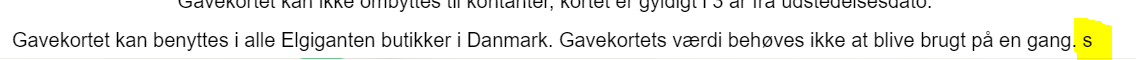
\includegraphics[height=1.5cm, width=17cm]{typo}
\end{center}
dette var indikator nok til at modtageren var skeptisk over for mailen. Dog endte personen med at klikke alligevel, da “den der tro og love erklæring gjorde mailen virkede troværdig nok til at den var ægte”.
\chapter*{4. Diskussion}
\addcontentsline{toc}{chapter}{4. Diskussion}
\noindent\textbf{Vishing}
\par Det som der var grundprincippet i telefonselskabets sikkerhed for at det kun er personen som er ejer af kontoen som kan få adgang og ændre oplysninger, er ved at bruge information som er meget personlig og ikke offentligt tilgængeligt. Hos Oister skulle der bruges det CPR nummer som er tilknyttet til kontoen før man kunne lave nogle ændringer, deres system tillod ikke medarbejdere at komme videre og foretage ændringer uden at et CPR nummer er opgivet. Dette er en utrolig god sikkerhedsforanstaltning, som også sikrer at selv hvis medarbejderen skulle være nemt påvirket af manipulation, tillader systemet ikke at medarbejderen kan komme videre med forespørgslen uden et CPR nummer. 

Havde der ikke været disse sikkerhedsforanstaltninger, ville man meget nemmere kunne ende med at have fuld kontrol over en anden konto. Og blandt andet få skiftet mailens kodeord og sikkerhedsspørgsmål for at gøre det rigtigt svært for den rigtige konto ejer at få adgang igen til sin egen konto. Dette ville give en angriber rigelig tid til at kunne prøve at få kortoplysninger som kunne være gemt på kontoen. Havde kontoen været forbundet til et online shopping side, som f.eks. Wish, som ikke har et to faktor check på kredit korts transaktioner hvor kreditkortet er gemt, havde det meget hurtigt kunne løbe op i mange penge som angriberen kunne bruge på bekostningen af en anden person.  

Et forsøg der kunne have været spændende at prøve, ville være at lave en ikke personlig vishing, og prøve at få et andet menneske til at give private oplysninger eller andet. Dog ville dette være umuligt at gøre på et lovligt grundlag, hvor personen stadig ikke er bevidst om hvad der foregår. 

\noindent\textbf{Vishing}
\par Tanken om, at man er sikker så længe man ikke giver oplysninger, er i visse tilfælde et godt udgangspunkt for en sikker indstilling. Dog er det ikke altid sikkert nok, da blot tanken om at klikke viser, at man har en vis tiltro til linket. Hvis den side man ender op på gennem linket ser troværdig ud, kan offeret hurtigt bliver manipuleret til at opgive oplysninger alligevel, da siden ligner det firma den udgiver sig for at være. Der er visse indikatorer der kan vise om hvorvidt et link er sikkert eller ej, men som udgangspunkt er det sikreste, at man ikke må klikke på links man ikke kender. På denne måde sikrer man sig også, at der ikke forekommer man-in-the-middle angreb, da størstedelen forekommer gennem disse phishing links.

At kigge på afsenderens mail adresse er også en god måde til at vurdere sikkerheden på indholdet og de medsendte links. Som tidligere skrevet var der flere af de personer vi sendte mailen til der kiggede på afsenders mail, som var en helt normal gmail. Det som kunne snyde her var, at gmail viser navnet på ejeren af mailen - som vi havde navngivet til Elgigant Teknik. 
\begin{center}
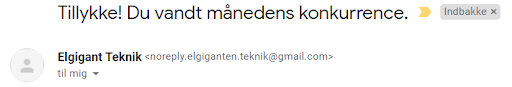
\includegraphics[height=2.3cm, width=17cm]{emailTitle}
\end{center}

Det er ikke alle der fanger det, men det er en tydelig indikator på, at der er noget galt at mailen ikke er fra firmaets egen domæne, for eksempel xxx@elgiganten.dk og i stedet en privat mail. Det betyder at man også, sammen med tidligere nævnte metoder, bør tage højde for hvem afsenderen er baseret på mail adressen.

De resultater vi fik fra vores forsøg viste ikke, at en bestemt aldersgruppe var mere tilbøjelig til at klikke på linket i mailen. Vel at mærke kan vi ikke konkludere om alder har en betydning, da datasættet vi har benyttet os af, er for småt. Vi kan dog konkludere, at generel viden omkring hvordan data transaktioner fungerer, samt forståelse for usikkerhed på nettet har betydning for, hvorvidt folk klikker på links de ikke kender eller ej. Det er dog, som tidligere skrevet, svært at drage en konklusion om, hvorvidt der er en sammenhæng mellem alder og chance for at klikke på et usikkert link.

Uanset alderen, kan dette problem løses ved blot at informere alle folk om, hvordan de bør tage hånd om links og andre usikre ting på internettet. Dermed har dette forsøg også været med til at give alle medvirkende personer en større forståelse om, hvorvidt en mail der ser autentisk ud, kan være ondsindet.

Den typo fejl der opstod i en af mailene var reelt set en fejl, men det er en god pointe at indføre såvel som de andre, da phishing mails har tendens til at have stavefejl og andre småfejl. Dette bør man også være opmærksom på, da det er et tydeligt tegn på u-professionalitet at have sådanne fejl med i en mail, og typisk indikerer at det nok ikke er hvad det udgiver sig for at være. Dette kan dog også forekomme ved oversættelsesfejl, da der er mange udenlandske firmaer der prøver at phishe på denne måde.

\chapter*{5. Konklusion}
\addcontentsline{toc}{chapter}{5. Konklusion}
Det er ikke alle der fanger det, men det er en tydelig indikator på, at der er noget galt at mailen ikke er fra firmaets egen domæne, for eksempel xxx@elgiganten.dk og i stedet en privat mail. Det betyder at man også, sammen med tidligere nævnte metoder, bør tage højde for hvem afsenderen er baseret på mail adressen.

De resultater vi fik fra vores forsøg viste ikke, at en bestemt aldersgruppe var mere tilbøjelig til at klikke på linket i mailen. Vel at mærke kan vi ikke konkludere om alder har en betydning, da datasættet vi har benyttet os af, er for småt. Vi kan dog konkludere, at generel viden omkring hvordan data transaktioner fungerer, samt forståelse for usikkerhed på nettet har betydning for, hvorvidt folk klikker på links de ikke kender eller ej. Det er dog, som tidligere skrevet, svært at drage en konklusion om, hvorvidt der er en sammenhæng mellem alder og chance for at klikke på et usikkert link.

Uanset alderen, kan dette problem løses ved blot at informere alle folk om, hvordan de bør tage hånd om links og andre usikre ting på internettet. Dermed har dette forsøg også været med til at give alle medvirkende personer en større forståelse om, hvorvidt en mail der ser autentisk ud, kan være ondsindet.

Den typo fejl der opstod i en af mailene var reelt set en fejl, men det er en god pointe at indføre såvel som de andre, da phishing mails har tendens til at have stavefejl og andre småfejl. Dette bør man også være opmærksom på, da det er et tydeligt tegn på u-professionalitet at have sådanne fejl med i en mail, og typisk indikerer at det nok ikke er hvad det udgiver sig for at være. Dette kan dog også forekomme ved oversættelsesfejl, da der er mange udenlandske firmaer der prøver at phishe på denne måde.
\chapter*{6. Bilag}
\addcontentsline{toc}{chapter}{6. Bilag}
\begin{figure}[H]
  \center{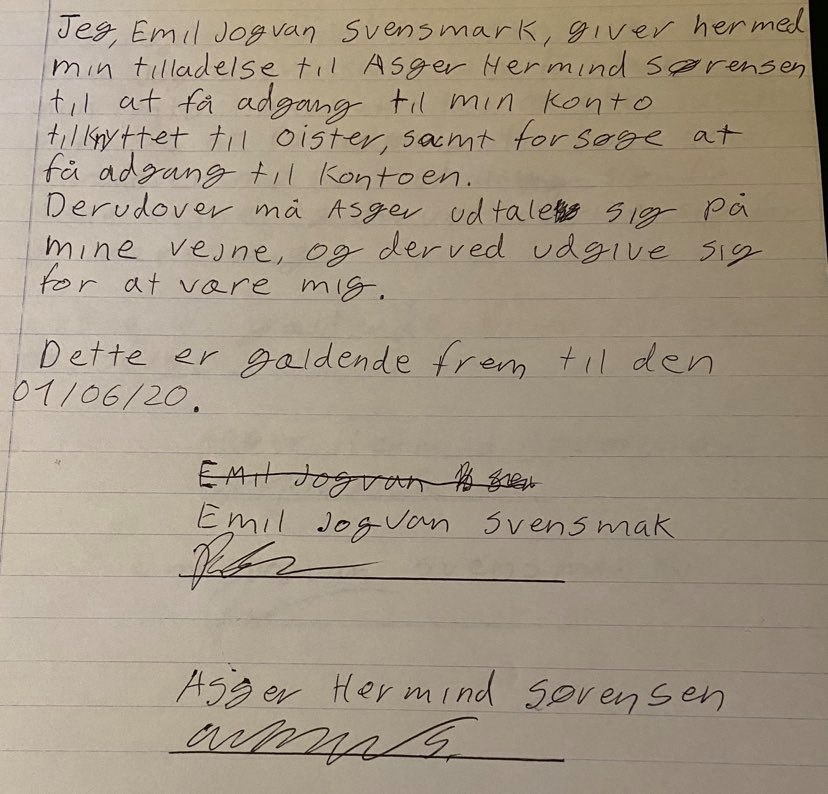
\includegraphics[height=12cm, width=17cm]
  {EmilKontrakt}}
  \caption*{1. Emils Kontrakt for tilladelse af vishing.}
\end{figure}
\begin{figure}[H]
  \center{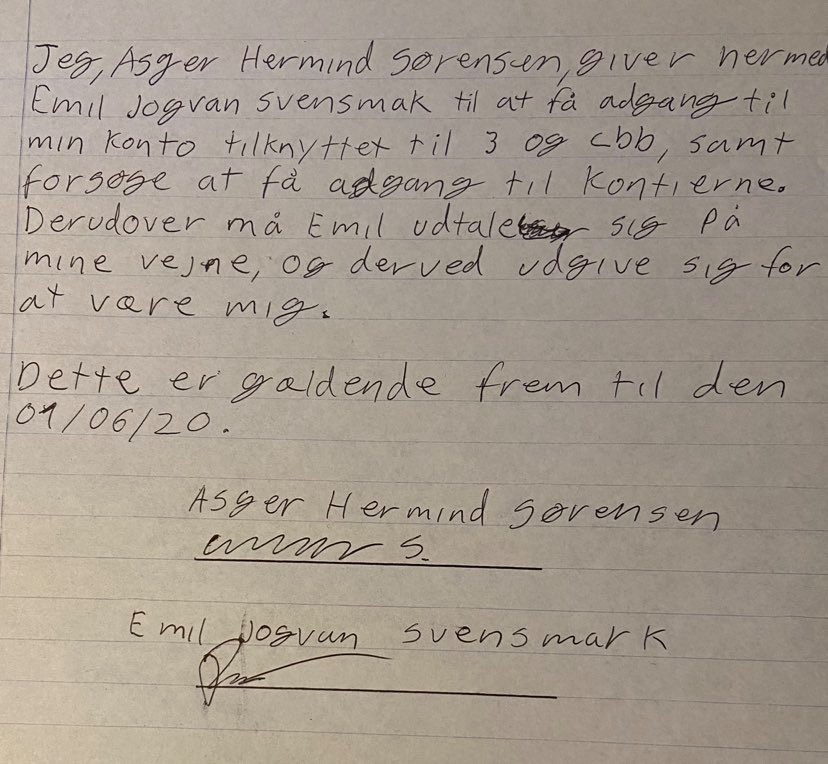
\includegraphics[height=12cm, width=17cm]
  {AsgerKontrakt}}
  \caption*{2. Asgers Kontrakt for tilladelse af vishing.}
\end{figure}

\end{document}